%-----------------------------------------------------------------------------------------------
\documentclass[addpoints, 11pt]{exam}
\usepackage[margin=.75in]{geometry}
\usepackage{etex}
\usepackage{graphicx}
\usepackage{amssymb}
\usepackage[fleqn]{amsmath}
\usepackage{nccmath}
\usepackage{cases}
\usepackage{hyperref}
\usepackage{multicol}
\usepackage{enumerate}
\usepackage{tikz}
\usepackage{pgfplots}
\usetikzlibrary{patterns}
\usepackage{pstricks-add}
%\usepackage{pst-func}
%\usepackage{pst-plot}
%\usepackage{pst-spectra}
\usepackage{multido}
\usepackage{lastpage}
\usepackage{ulem}
\usepackage[outside]{coordsys}
\usepackage{float}
\usetikzlibrary{pgfplots.statistics}
\usetikzlibrary{positioning, shapes.geometric}
%-------------------------------------------------------------------------------------------------
\setlength{\columnsep}{.5cm}
\setlength{\columnseprule}{1pt}
\newcommand{\ds}{\displaystyle}
\newcommand{\work}{{\bf{No Work $\Leftrightarrow$ No Points }}}
\newcommand{\neat}{{\bf{Use Pencil Only $\Leftrightarrow$ Be Neat \& Organized }}}
\newcommand{\answer}{\large\bf Ans: \underline{\hspace{1.5in}}}
\newcommand{\la}{\lambda}
\newcommand{\zz}{\mathbb{Z}}
\newcommand{\rr}{\mathbb{R}}
\newcommand{\nn}{\mathbb{N}}
\newcommand{\qq}{\mathbb{Q}}
\newcommand{\cc}{\mathbb{C}}
\newcommand{\cyclic}[1]{\langle #1 \rangle}
\newcommand{\lcm}{{\rm{lcm}}}
\renewcommand{\solutiontitle}{\noindent\textbf{Answer:}\par\noindent}
%------------------------------------------------------------------------------------------------
\begin{document}
%------------------------------------------------------------------------------------------------
\cfoot{UCLA: C. Johnson}
%	\rfoot{Total Points: \numpoints}
\rfoot{Page \thepage\ of \pageref{LastPage}}
%------------------------------------------------------------------------------------------------
\begin{center}
\fbox{%
	\parbox{1\linewidth}{%
		\noindent \Large\bfseries \\[.05in] Math 142: Modeling{\hspace{1.2in}{\Large\bfseries Name:{\hrulefill}}\\[.2cm]
			\noindent \Large\bfseries Homework \# 7 \hspace{2.8in}{Due:} Monday Dec 4
		}\\[.025in]
	}%
}
\end{center}
\addpoints


\vspace{.25cm}


%------------------------------------------------------------------------------------------------
\noindent  {\bf Directions} Complete the exercises. Your solutions to the exercises should be submitted to Gradescope before the indicated due date above. Please follow rules regarding Gradescope submission as described in the syllabus. \\


\noindent{\bf References} Except for the help of the instructor or TAs and the class textbooks and notes, if you use any resources, for example, a book, a website, or you discussed with your friends, please acknowledge them in this References section. 
\begin{itemize}
\item I discussed Problem ?? with STUDENT A, STUDENT B, $\ldots$
\item I used BOOK/WEBSITE to help me do Problem ??.
\end{itemize}
\vspace{.05cm}
%\hrule
%----------------------------------------------------------------------------------------------  
\noindent {\bf Exercises}
%\begin{multicols*}{2}
\begin{questions}
%----------------------------------------------------------------------------------------------  
\question  A set of bacteria obey the continuum hypothesis if the number of bacteria in an interval is proportional the size of the interval, so long as the interval size is not too large and not too small. The uploaded Matlab file nonuniformswimmers.mat contains coordinates (generated on a computer) for 500 swimmers that are randomly (and not uniformly) distributed over the interval $0 \leq x \leq 1$
\begin{parts}
	\part Make a graph of the number of swimmers contained in the interval: $\frac{1}{2}-\frac{\Delta x}{2}<x<\frac{1}{2}+\frac{\Delta x}{2}$, as a function of the interval length $\Delta x$, and estimate the range of $\Delta x$ over which the number is proportional to $\Delta x$.
	\begin{figure}[H]
		\centering
		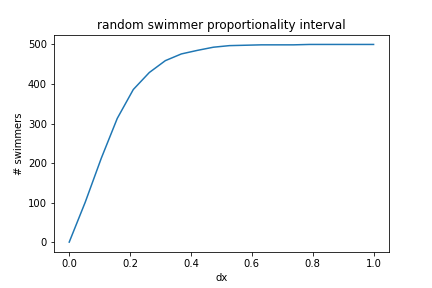
\includegraphics[scale=0.5]{random swimmer proportionality interval.png}
	\end{figure}
	range of proportional interval lengths $\approx 0.01-0.2$
	\part Estimate the density of swimmers $\rho(1 / 2)$ (note there is no time dependence, because the swimmers aren't moving around).\\
	$\rho(1/2)\approx 2000$
	\part Explain why, if instead of being distributed as given in this question, all of the bacteria were located at $x=1 / 2$, their distribution would not obey the continuum hypothesis.\\
	The number of bacteria contained in the interval would be constant for all $\Delta x>0$
\end{parts}
%----------------------------------------------------------------------------------------------   
\question In this question you will work with the conservation law:
$$
\frac{\partial \rho}{\partial t}+\frac{\partial q}{\partial x}=0 .
$$
assuming in each part, different densities $\rho$ and flow rates $q$.
\begin{parts}
	\part Assume that $\rho(x, t)=x+t$ and $q(x, t)=t-x$. Is the conservation law satisfied?\\
	$\frac{\partial \rho}{\partial t}=1,\frac{\partial q}{\partial x}=-1\Rightarrow \frac{\partial \rho}{\partial t}+\frac{\partial q}{\partial x}=0$. Yes
	\part Assume that $\rho(x, 0)=x$ and $q(x, t)=x^2+t^2$. Find $\rho(x, t)$.\\
	$\frac{\partial q}{\partial x}=2x\Rightarrow \frac{\partial \rho}{\partial t}=-2x\Rightarrow \rho(x,t)=-2xt+f(x)$. Given $\rho(x, 0)=x$, $\rho(x,t)=-2xt+x$.
	\part Assume that $\rho(x, t)=\sin (x+t)$. Find $q(x, t)$. Your answer will include an unknown function of time - what additional information would you need to know in order to completely solve for $q(x, t)$ ?\\
	$\frac{\partial \rho}{\partial t}=\cos(x+t)\Rightarrow \frac{\partial q}{\partial x}=-\cos(x+t)\Rightarrow q(x,t)=-\sin(x+t)+f(t)$. 
\end{parts}
%----------------------------------------------------------------------------------------------   
\question Consider the diffusion equation:
$$
\frac{\partial \rho}{\partial t}=D \frac{\partial^2 \rho}{\partial x^2}
$$
modeling the diffusion of bacterial within a channel $0<x<1$. Assume that end $x=0$ is closed, and that end $x=1$ is open to a large chamber.
\begin{parts}
	\part What boundary conditions should we use at the two channel ends? Justify how the boundary conditions represent the scenarios of closed or open channel ends.\\
	At $x=0$, the end is closed, so there can no net flux at $x=0$. Thus, $q(0,t)=0$ and $-D\rho_x=0$ at $x=0$. At $x=1$, the end is open, so the bacteria disapear when the reach the open end. Thus, $\rho(1,t)=0$
	\part Show that if the total number of bacteria in the channel is $N(t) \equiv \int_0^1 \rho(x, t) d x$, then $\frac{d N}{d t}=-q(1, t)$\\
	$\frac{d N}{d t}=\frac{\partial \int_0^1 \rho(x, t) d x}{\partial t}=\int_0^1\frac{\partial\rho}{\partial t}dx=-\int_{0}^{1}\frac{\partial q}{\partial x}dx=-q(1,t)+q(0,t)=-q(1,t)$ because $q(0,t)=0$.
	\part Explain why $q(1, t) \geq 0$, (i) in terms of what we expect bacteria to do at the open end of the channel and (ii) mathematically by considering the sign of $\frac{\partial \rho}{\partial x}$.\\
	(i) There are no bacteria to the right of $x=1$, so the the net flow rate must be from left to right.\\
	(ii) $\frac{\partial \rho}{\partial x}\le 0$ because the pressure would be decreasing at a point where bacteria can leave, so $q=-D\frac{\partial \rho}{\partial x}\ge0$.
\end{parts}
%---------------------------------------------------------------------------------------------- 
\question Bacteria swim randomly around in a channel $-1<x<1$, with diffusivity $D$. They also divide, with both rate $b$ (you can assume that mortality is so small that it can be neglected).
\begin{parts}
	\part Assume that the two ends of the channel are closed. Write down an associated PDE and boundary conditions. Using Matlab (with any initial condition you like) or your intuition, try to explain why you would expect $\rho(x, t) \rightarrow \rho(t)$ as $t \rightarrow \infty$. That is, at late times, the density is uniform in $x$ but varies with $t$. Assuming that there are initially $N_0$ bacteria in the channel, find the function $\rho(t)$.\\
	$\frac{\partial \rho}{\partial t}+\frac{\partial q}{\partial x}=b\rho(x,t)$ with boundary conditions $q(-1,t)=0$ and $q(1,t)=0$.\\
	$\frac{\partial \rho}{\partial t}-b\rho(x,t)=D\frac{\partial^2 \rho}{\partial x^2}$\\
	$\Rightarrow\rho(x,t)=De^{bt}\int e^{-bt}\frac{\partial^2 \rho}{\partial x^2}dt\Rightarrow \rho(t)\propto e^{bt}$. 
	intuititively, the population will diffuse in the shape of a bell curve, but because the bacteria can't swim past the ends of the channel, more bacteria will collect at the ends of the channel than would be modeled by a bell curve. In the limit, the population will appear uniform.
	\part Now assume the two ends of the channel are open, and that $b=1$. Using the ICs: $\rho(x, 0)=$ 10 if $|x|<0.1$ and $\rho(x, 0)=0$ otherwise, and Matlab find the behavior of $\rho(x, t)$ for small diffusivity $D=0.1$, and for moderate diffusivity $D=1$. Can you explain in words, why different diffusivities produce very different behaviors?\\
	If the bacteria are reproducing faster than the bacteria are leaving the channel, then the density will increase $\frac{\partial \rho}{\partial t}>0$ for all x in the channel, but if the diffusivity rate is high enough, the density will go to $0$.
\end{parts}
%----------------------------------------------------------------------------------------------
\question We discussed in class that the total heat energy in length $\Delta x$ of a bar is given by $\rho c_p T \Delta x$, and the total flow of heat obeys $q=-k A \frac{\partial T}{\partial x}$. The bar occupies the length $0<x<L$. Here $A$ is the cross-section area of the bar and $\rho c_p, k$ are positive constants.
\begin{parts}
	\part Assume that the end $x=1$ is heated to a constant temperature $T=1$. The end $x=0$ is insulated, so that heat neither leaves nor enters the bar there. What mathematical boundary conditions should be used to model the two ends of the bar?\\
	At $x=0$, the heat can't escape or enter the insulated end, so $q(0,t)=0$. At $x=1$, any heat that escapes the end at $x=1$ is imediately replaced because the end is being heated to a constant temperature, so $T(1,t)=1$.
	\part The bar loses heat to the surrounding air. Newton's law of cooling says that a length $\Delta x$ of bar will lose energy at a rate $-\sigma A T \Delta x$, where $\sigma$ is another positive constant. Explain how to modify our conservation of heat energy equation to include heat lost to the air.\\
	We can modify the equation to be $\frac{\partial A\rho c_p T}{\partial t}+\frac{\partial q}{\partial x}=-\sigma A T$
	\part Assume that as $t \rightarrow \infty, T \rightarrow T(x)$, a steady temperature. Find this steady temperature. (Hint: it may help to write the solution of the ODE in terms of $\sinh$ and $\cosh$ - speak to us in office hours if you don't know these functions).\\
	$\frac{\partial A\rho c_p T}{\partial t}+\frac{\partial q}{\partial x}=-\sigma A T\Rightarrow \frac{\partial A\rho c_p T}{\partial t}+\sigma A T=kA\frac{\partial^2 T}{\partial x^2}\Rightarrow \frac{\partial \rho c_p T}{\partial t}+\sigma  T=k\frac{\partial^2 T}{\partial x^2}$. As $T\rightarrow T(x)$, $\frac{\partial T}{\partial t}\rightarrow 0$, so $\frac{\partial \rho c_p T}{\partial t}+\sigma  T=k\frac{\partial^2 T}{\partial x^2}\Leftrightarrow \sigma T=k\frac{\partial^2 T}{\partial x^2}\Rightarrow T(x)=c_0\sinh(\sqrt{\frac{\sigma}{k}}x)+c_1\cosh(\sqrt{\frac{\sigma}{k}}x)\Rightarrow T(x)=\frac{1}{\cosh(\sqrt{\frac{\sigma}{k}})}\cosh(\sqrt{\frac{\sigma}{k}x})$ given the boundary conditions.
\end{parts}
%----------------------------------------------------------------------------------------------
\question  Morphogens are molecules that direct differentiation in developing embryos. That is they tell cells and nuclei what parts of the organism they should become. Early in embryo development the embryo has an ellipsoid shape, like an American football. Morphogens are produced at the poles (pointy ends) of the football at diffuse from there into the interior. Let $c(x, t)$ be the concentration of morphogen per unit length of embryo.

Assume that we can treat this process as a 1D reaction diffusion equation, with the poles of the football at $x=\pm L$. Assume that the morphogens diffuse into the embryo with diffusivity $D$. As they diffuse into the embryo they are broken down within the cells they pass through. Assume that a unit length of tissue breaks down morphogen at a rate $\lambda$. Assume that the poles each produce morphogen at rate $Q$.
\begin{parts}
	\part Find the PDE to describe the morphogen diffusion into the tissue, and present its boundary conditions.\\
	$\lambda c(x,t)+\frac{\partial c}{\partial t}=D\frac{\partial^2 c}{\partial x^2}$ with boundary conditions $c(L,t)=c(-L,t)=0$ and $q(L,t)=q(-L,t)=0$.
	\part Assume that the concentration approaches some steady state $c(x,t) \rightarrow c(x)$ as $t \rightarrow \infty$. Find this steady state.\\
	As $c(x,t) \rightarrow c(x)$, $\frac{\partial c}{\partial t}\rightarrow 0$. It follows $c(x)=\frac{D}{\lambda}\frac{\partial^2 c}{\partial x^2}\Rightarrow c(x)=c_0\sinh(\sqrt{\frac{\lambda}{D}}x)+c_1\cosh(\sqrt{\frac{\lambda}{D}}x)\Rightarrow c(x)=0$ given the boundary conditions. ($0=c_0\sinh(\sqrt{\frac{\lambda}{D}}L)+c_1\cosh(\sqrt{\frac{\lambda}{D}}L), 0=c_0\sqrt{D\lambda}\cosh(\sqrt{\frac{\lambda}{D}}L)+c_1\sqrt{D\lambda}\sinh(\sqrt{\frac{\lambda}{D}}L)$)
\end{parts}
%----------------------------------------------------------------------------------------------
\question Practice with advective derivatives
\begin{parts}
	\part Traffic on a freeway has a steady density field $\rho(x, t)=\alpha x$ where $\alpha<0$. A motorcyclist rides on the hard shoulder at speed $v$.
	First explain in words, and then verify by calculating an advective derivative: Is the density field observed by the motorcyclist increasing, decreasing, or stationary if: (i) $v=0$ (ii) $v>0$ ?\\
	(i) when the motorcyclist is stationary, the freeway doesn't appear to be moving because the freeway density is stationary i.e doesn't depend on time.\\
	(ii) when the motorcyclist is moving, the freeway appears to be moving backward because the freeway is stationary.\\
	$q(\rho)_x+\rho_t=0\Rightarrow \frac{\partial q}{\partial \rho}\frac{\partial \rho}{\partial x}+\frac{\partial \rho}{\partial t}=0\Rightarrow \frac{\partial q}{\partial \rho}=0$ because $\frac{\partial \rho}{\partial t}=0$ and $\frac{\partial \rho}{\partial x}=\alpha$.\\
	Using change of variables $\tilde{x}=x-vt$ and $\tilde{t}=t$.\\
	$\frac{\partial\rho}{\partial x}=\frac{\partial \rho}{\partial \tilde{x}}\frac{\partial \tilde{x}}{\partial x}+\frac{\partial \rho}{\partial \tilde{t}}\frac{\partial \tilde{t}}{\partial x}=\alpha$ and $\frac{\partial\rho}{\partial t}=\frac{\partial \rho}{\partial \tilde{x}}\frac{\partial \tilde{x}}{\partial t}+\frac{\partial \rho}{\partial \tilde{t}}\frac{\partial \tilde{t}}{\partial t}=-v$\\
	It follows $\frac{\partial q}{\partial \rho}\frac{\partial \rho}{\partial \tilde{x}}+\frac{\partial \rho}{\partial \tilde{t}}=\frac{\partial q}{\partial \rho}(\alpha)-v=0\Rightarrow \frac{\partial q}{\partial \rho}=\frac{v}{\alpha}$, so $\frac{\partial q}{\partial \rho}=0$ for $v=0$ and $\frac{\partial q}{\partial \rho}<0$ when $v>0$.
	\part We know that linearized traffic flow obeys an equation: $\frac{\partial \rho_1}{\partial t}+c \frac{\partial \rho_1}{\partial x}=0 \mathrm{By}$ substituting into the equation show that if $g$ is any differentiable function then $\rho_1(x, t)=g(x-c t)$ will obey the linearized traffic flow equation.\\
	$\frac{\partial \rho_1}{\partial t}=-c\cdot g'(x-ct),\frac{\partial \rho_1}{\partial x}=g'(x-ct)\Rightarrow \frac{\partial \rho_1}{\partial t}+c \frac{\partial \rho_1}{\partial x}=-c\cdot g'(x-ct)+c\cdot g'(x-ct)=0$
\end{parts}
%----------------------------------------------------------------------------------------------
\question We may assume that cars on a particular freeway obey the Greenshields' model. We choose our units so that $u_{\max }=1$ and $\rho_{\max }=1$. Suppose that the initial density of cars is given by $\rho(x, t)=\rho_0+\epsilon \rho_1(x, t)$.
\begin{parts}
	\part Assuming $\epsilon \ll 1$, and starting from the Lighthill Whitham Richards equation:
	$$
	\frac{\partial \rho}{\partial t}+\frac{\partial}{\partial x} q(\rho)=0
	$$
	explain how to derive the linearized traffic flow equation for $\rho_1$ :
	$$
	\frac{\partial \rho_1}{\partial t}+c \frac{\partial \rho_1}{\partial x}=0
	$$
	$\frac{\partial \rho}{\partial t}=\epsilon\frac{\partial \rho_1}{\partial t}$. The Taylor expansion of $q$ around $p_0$ is $q(x)=\sum_{k=0}^{\infty}\frac{q^{(k)}(p_0)(x-p_0)}{k!}= q(p_0)+\frac{\partial q}{\partial x}|_{p_0}(x-p_0)+O(x-p_0)\Rightarrow \frac{\partial q}{\partial x}=\frac{\partial q}{\partial x}|_{p_0}+O(\epsilon p_1)\approx \frac{\partial q}{\partial x}|_{p_0}$ at $x=p_0+\epsilon p_1(x,t)$ because $p_0+\epsilon p_1(x,t)$ is very close to $p_0$.
	It follows we can express $\frac{\partial q(\rho)}{\partial x}=\epsilon\frac{\partial q}{\partial x}|_{p_0}\frac{\partial \rho_1}{\partial x}$\\
	This gives us $\epsilon\frac{\partial q}{\partial x}|_{p_0}\frac{\partial \rho_1}{\partial x}+\epsilon\frac{\partial \rho_1}{\partial t}=0\Rightarrow \frac{\partial q}{\partial x}|_{p_0}\frac{\partial \rho_1}{\partial x}+\frac{\partial \rho_1}{\partial t}=0$
	\part Assume that $\rho_0=\frac{1}{8}$. We are concerned about a traffic jam that is represented at $t=0$ by $\rho_1(x, 0)=1$ if $-1 \leq x \leq 1$, and $\rho_1(x, 0)=0$ otherwise. The traffic jam will clear when the density bump passes out of the freeway at $x=10$. Find the time at which the traffic jam is completely cleared.\\
	$q=\rho(1-\rho)\Rightarrow \frac{\partial q}{\partial \rho}|_{\rho_0}=1-\frac{1}{4}=\frac{3}{4}\Rightarrow t=\frac{4}{3}\cdot11=\frac{44}{3}$ because we want $\rho(x-\frac{3}{4}t)=0\Rightarrow x=11\Rightarrow t=\frac{44}{3}$
\end{parts}
%----------------------------------------------------------------------------------------------
%----------------------------------------------------------------------------------------------
\question Submit the code you used for any and all of the problems. (Print pdf the code) Either lump it all together at the end or when matching problems on Gradescope, select all pages of pdf that has code if you included code within the solution to each answer.
\begin{figure}[H]
	\centering
	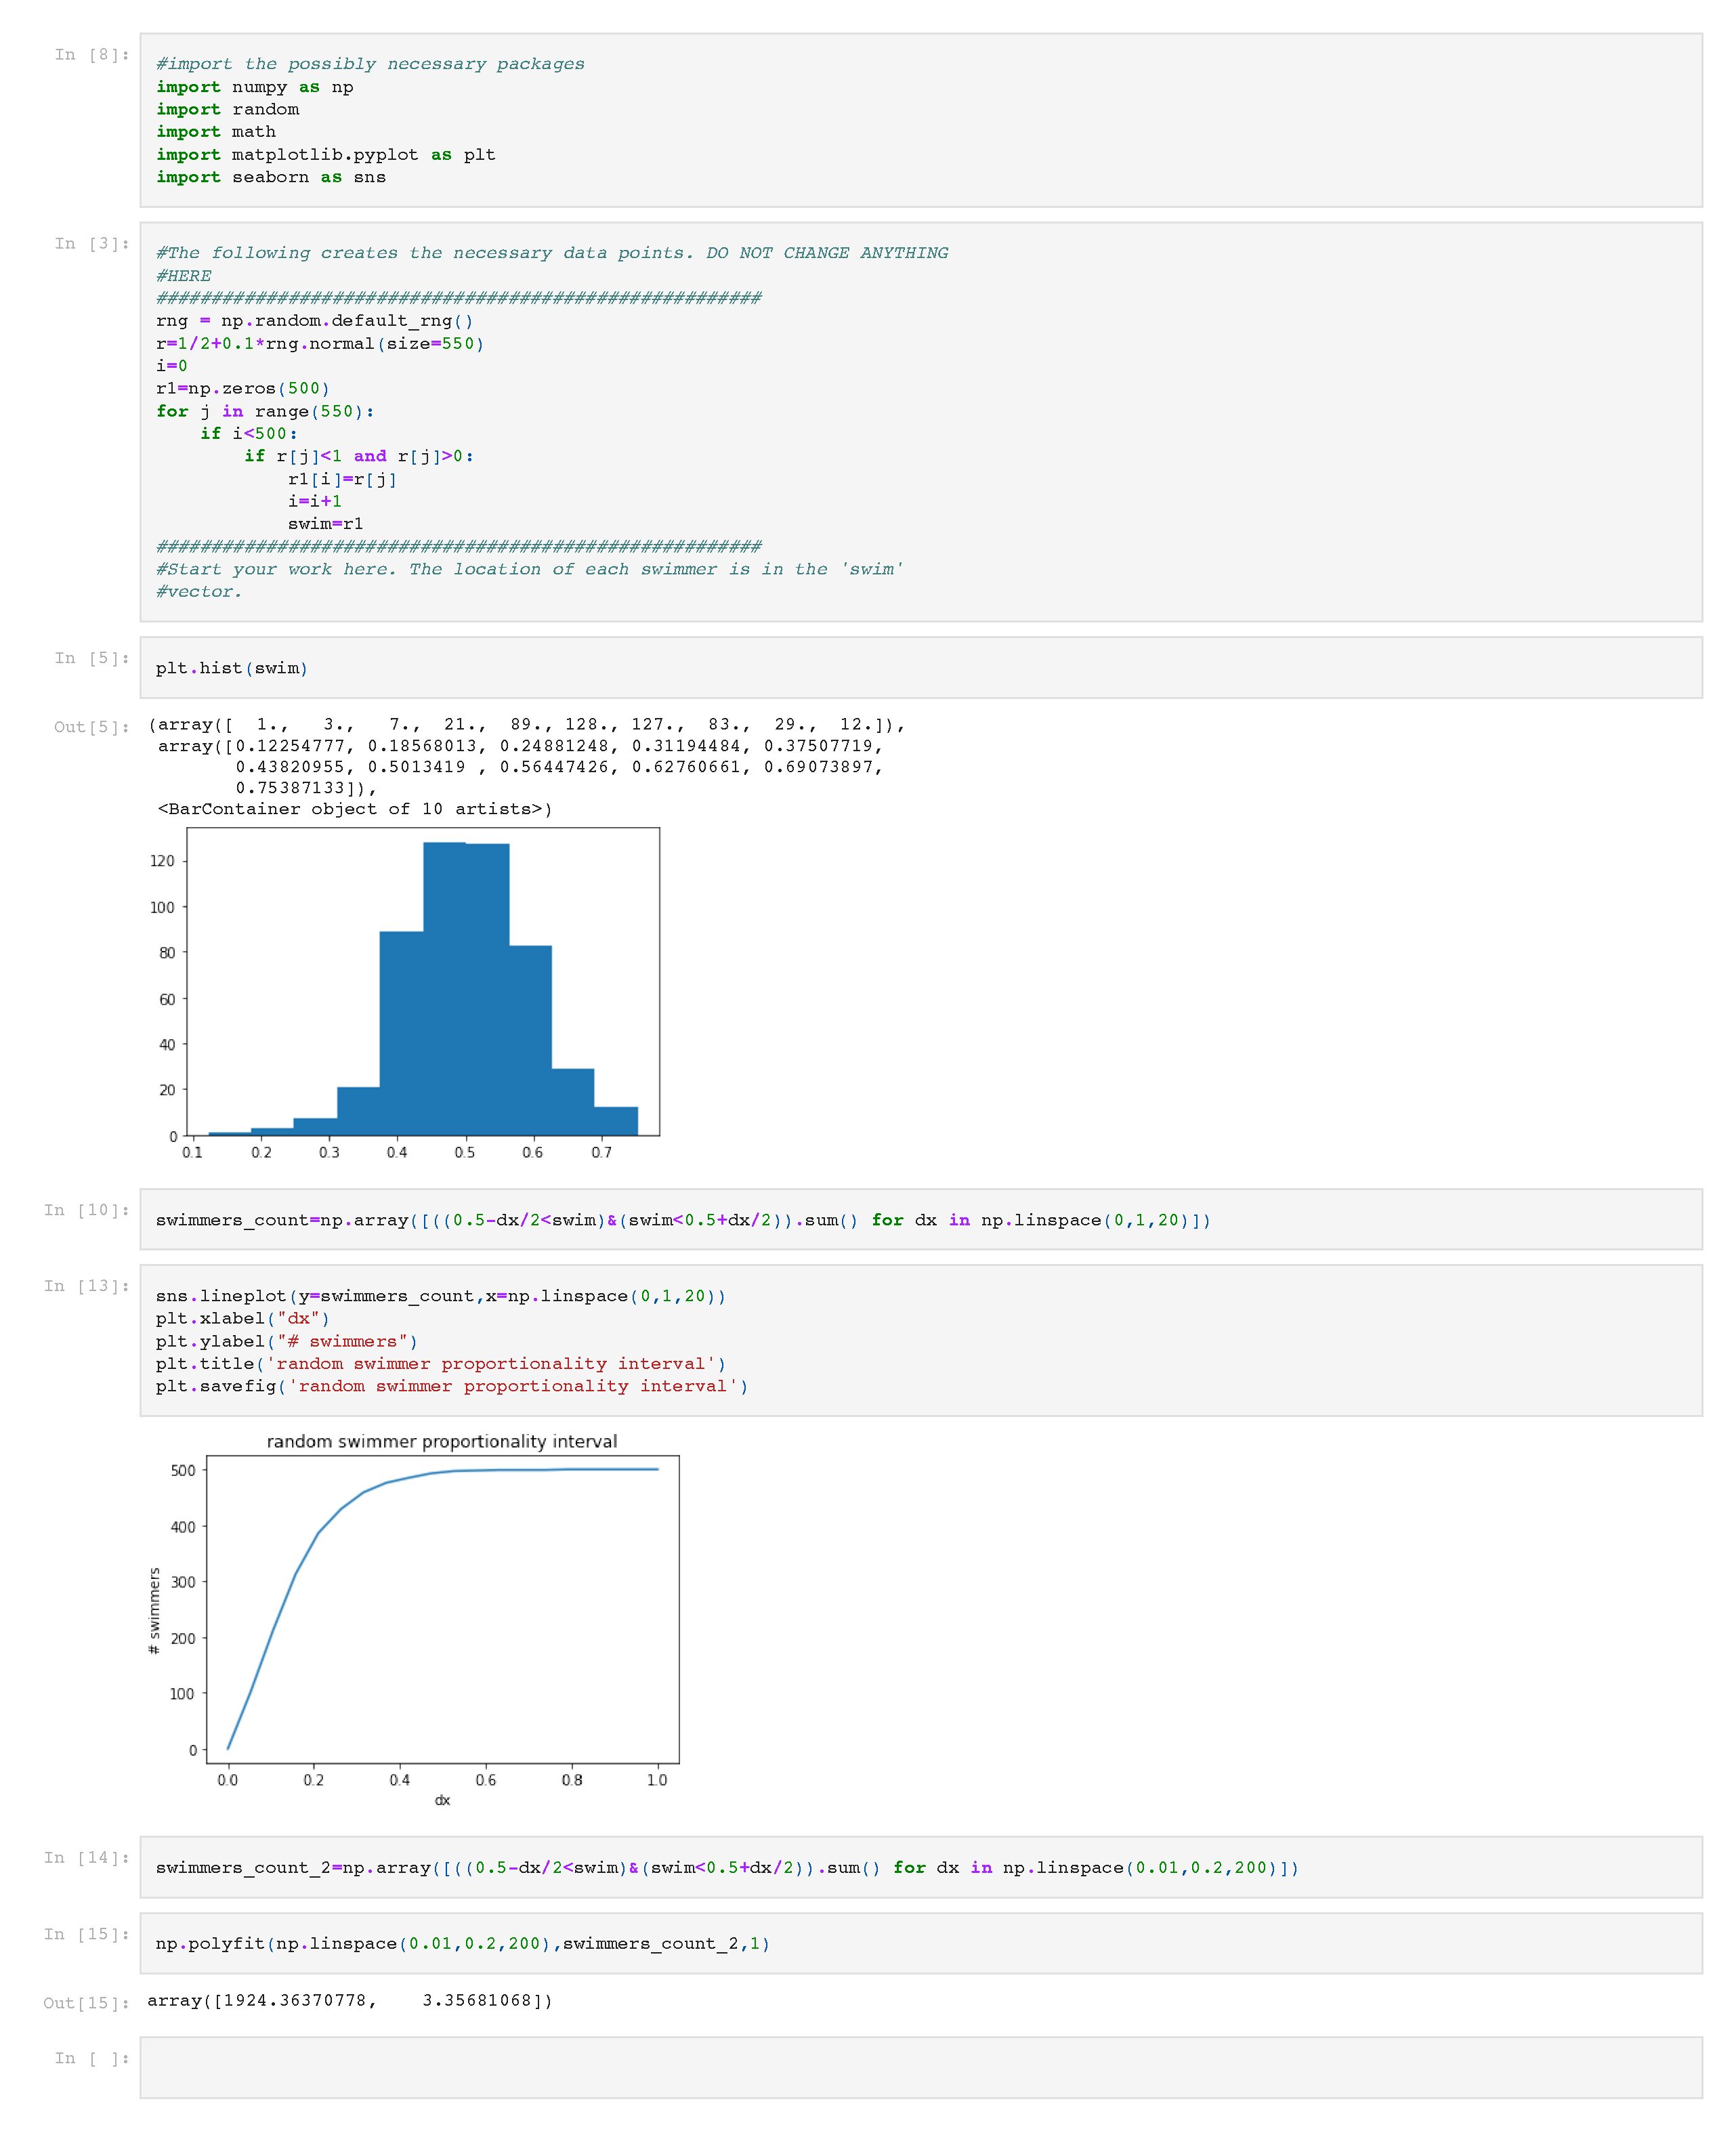
\includegraphics[scale=0.5]{Untitled7.pdf}
\end{figure}
%----------------------------------------------------------------------------------------------

\end{questions}
%\end{multicols*}
\end{document}